\chapter{Feature Maps Visualization} % Main appendix title
\label{AppendixC} % For referencing this appendix elsewhere, use \ref{AppendixA}

\newpage
%% feature maps comparison
\begin{figure}[H]
	\centering
	\captionsetup{width=\linewidth}
	\begin{subfigure}[b]{\linewidth}
		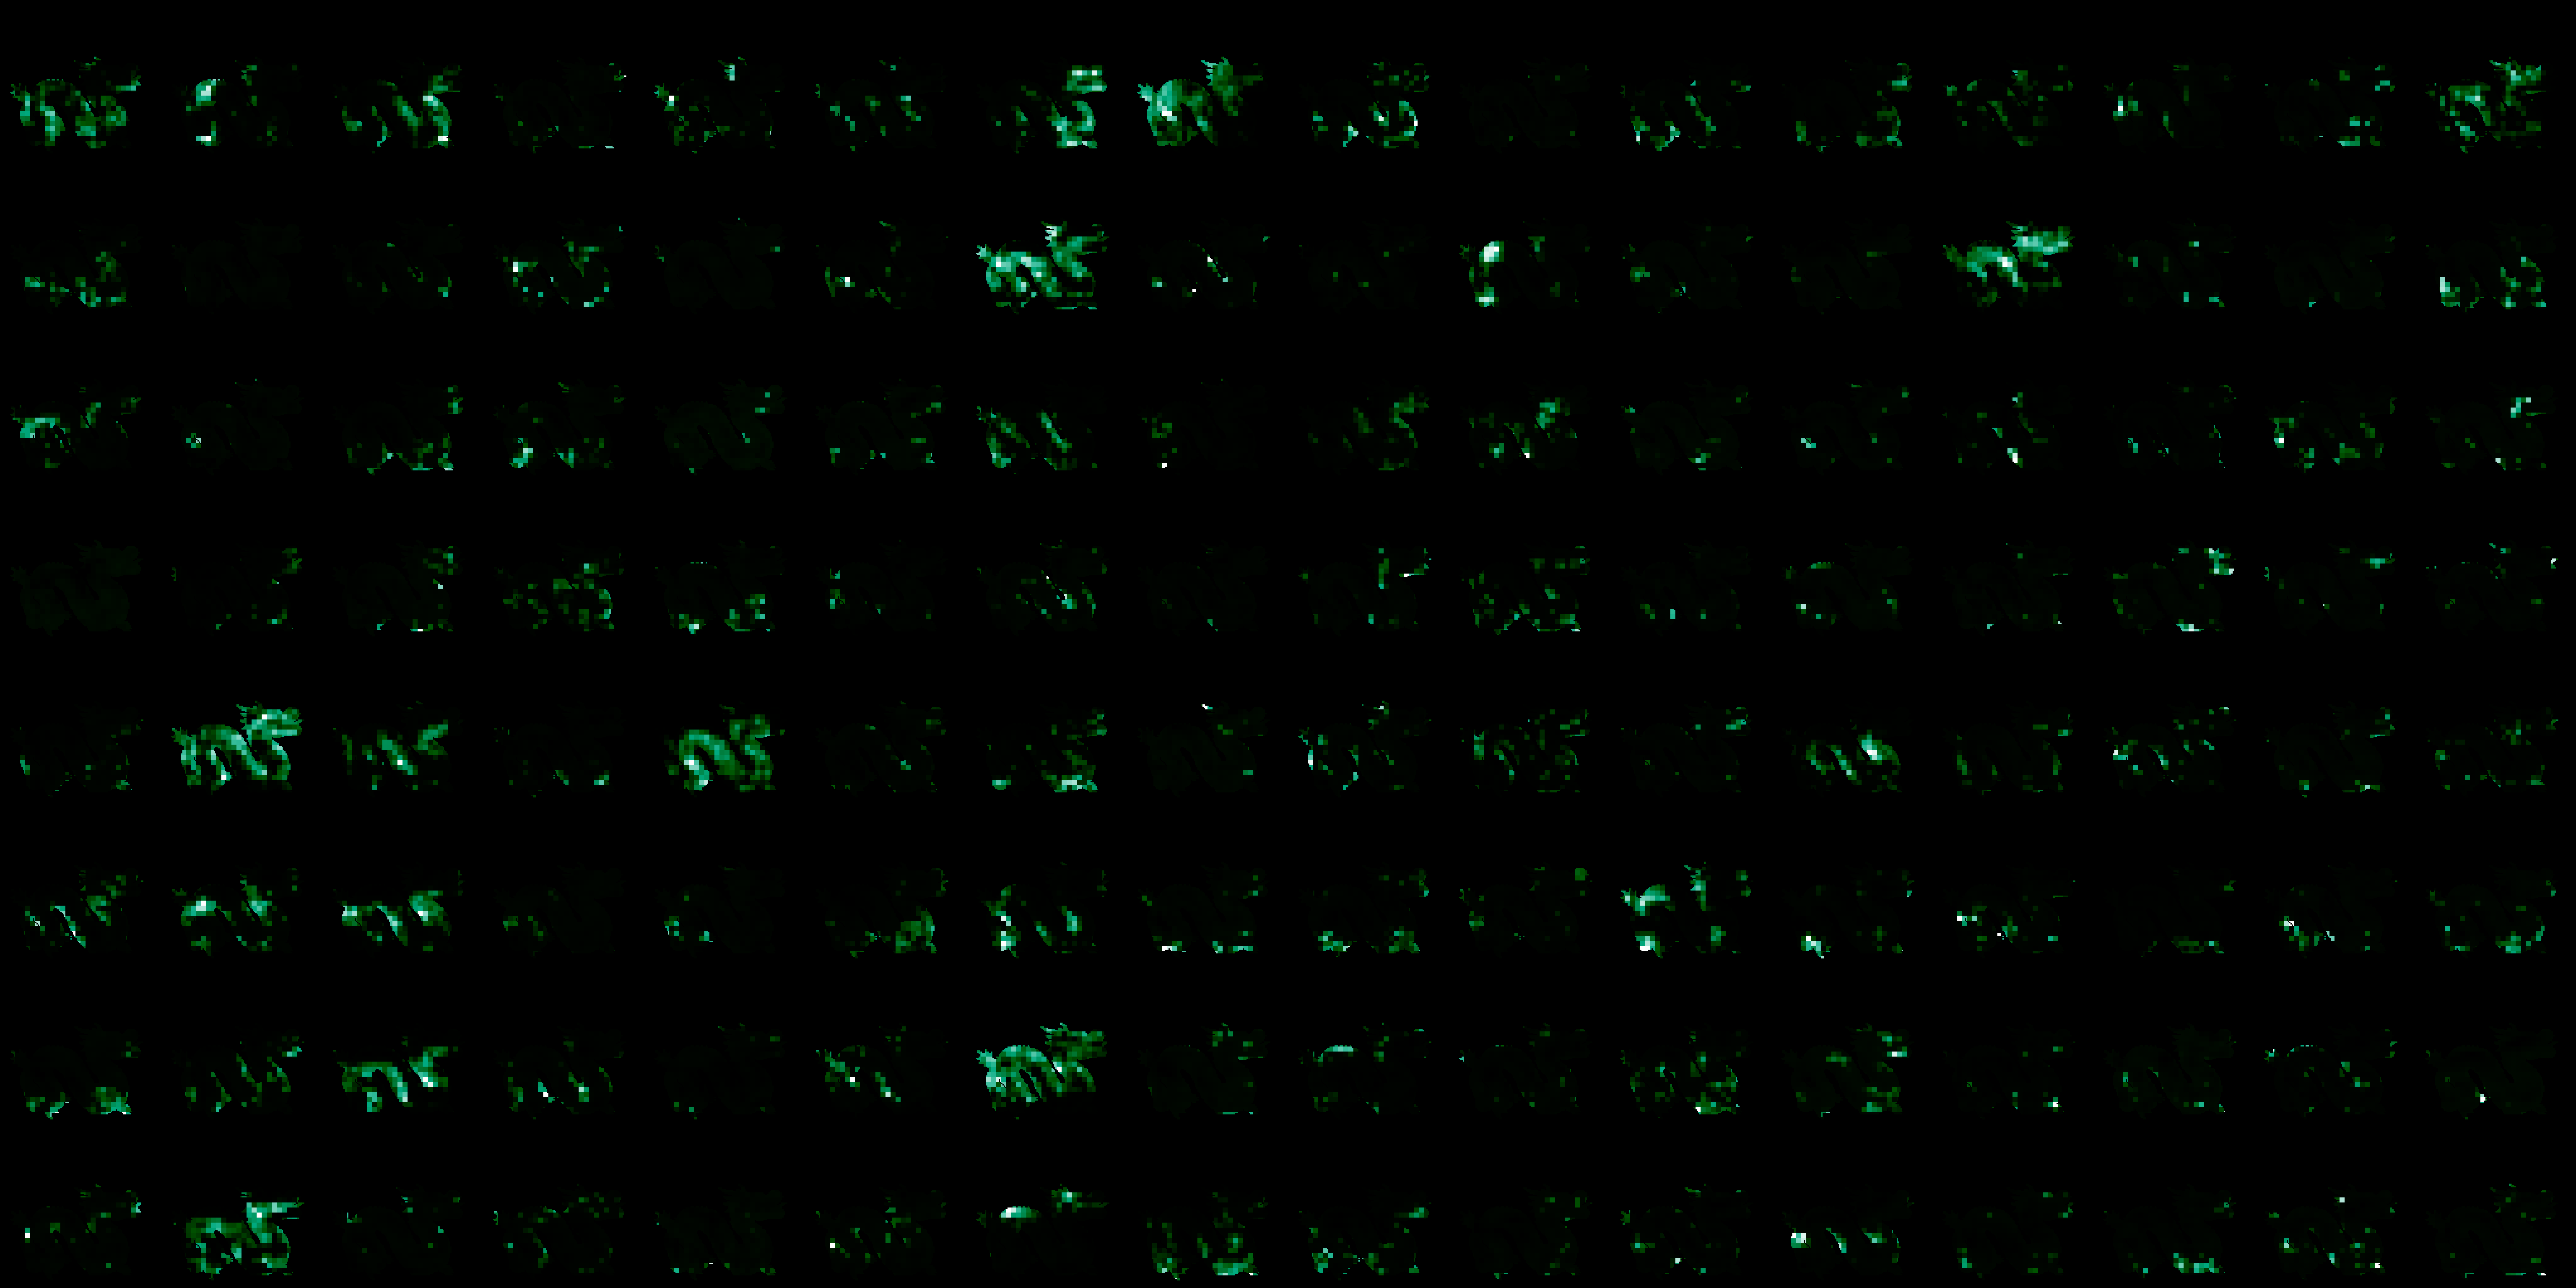
\includegraphics[width=\linewidth]{./Figures/feature_map_gcnn/feature_map_gcnn-cnn.png}
		\caption{CNN Feature Maps}
	\end{subfigure}
	
	\begin{subfigure}[b]{\linewidth}
		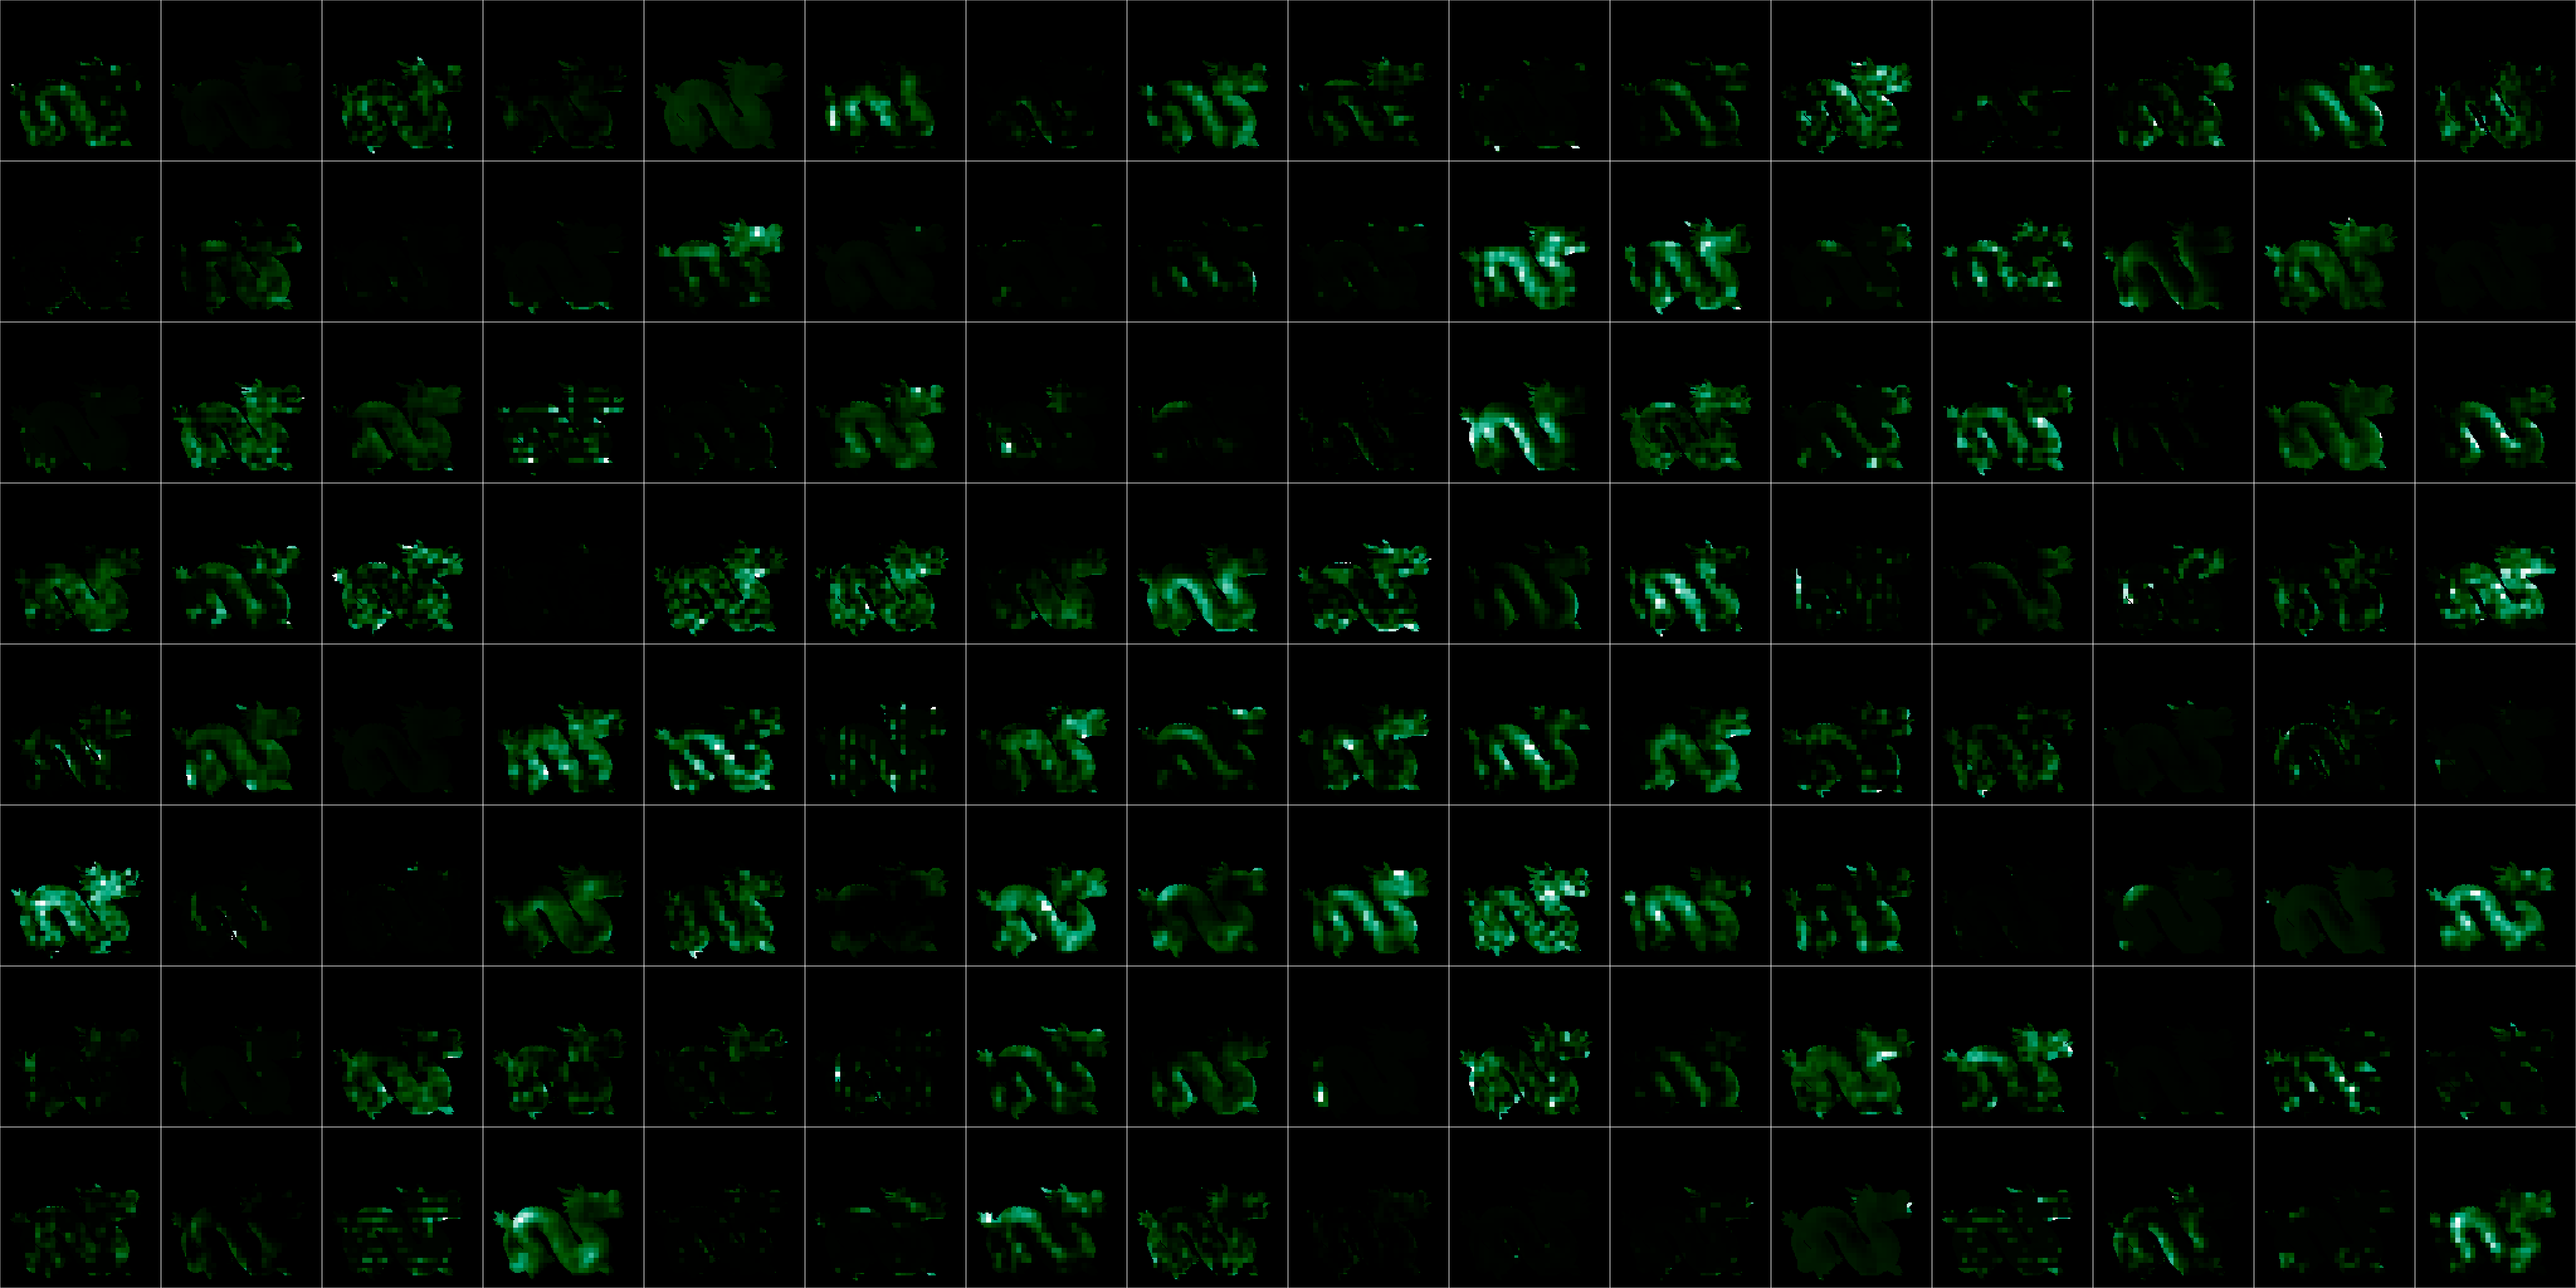
\includegraphics[width=\linewidth]{./Figures/feature_map_gcnn/feature_map_gcnn-noc.png}
		\caption{NOC Feature Maps}
	\end{subfigure}
	
	\begin{subfigure}[b]{\linewidth}
		\includegraphics[width=\linewidth]{./Figures/feature_map_gcnn/feature_map_gcnn-gcnn.png}
		\caption{GCNN Feature Maps}
	\end{subfigure}
	
	\begin{tikzpicture}
		\node[text width=0.1\textwidth] at (11,-1) {1};
		\node[inner sep=0pt] (input) at (8,-1)
		{
\includegraphics[width=.2\textwidth]{./Figures/colorscale_deepgreen.jpg}};
		\node[text width=0.3\textwidth] at (7,-1) {Value: 0};
	\end{tikzpicture}
	\decoRule
	\caption{All 128 Feature maps of model GCNN, NOC, CNN at the first up-sampling. (Resolution $ 32\times 32 $)}
	\label{fig:gcnn-cnn-feature map}
\end{figure}